\documentclass[aps,pra,twocolumn,reprint,amsmath,amssymb]{revtex4-2}

\usepackage{graphicx}
\usepackage{booktabs}
\usepackage{siunitx}
\usepackage[colorlinks=true,linkcolor=blue,citecolor=blue,urlcolor=blue]{hyperref}
\usepackage{float}
\usepackage{xcolor}

\begin{document}

\title{Runtime-Validated Hybrid Unitary Synthesis with Native Entangling Evolution}
\author{Execution Engineer}
\affiliation{cQED Autonomous Research Platform}
\date{\today}

\begin{abstract}
We revisit the previously defined hybrid qubit-cavity target unitary
$U_{\mathrm{target}} = (I_q \otimes H_c)\,\mathrm{CNOT}_{c \rightarrow q}\,\mathrm{CNOT}_{q \rightarrow c}$
on the logical subspace $\{\lvert g,0 \rangle, \lvert g,1 \rangle, \lvert e,0 \rangle, \lvert e,1 \rangle\}$
and convert an earlier symbolic-native-entangler conclusion into a runtime-backed
one. Symbolically, the exact two-wait architecture remains an upper bound with
process fidelity $0.9999998$, while the best experimentally grounded symbolic
candidate, the fully archive-driven two-wait family, reaches process fidelity
$0.98568$. To close the replay gap inside \texttt{cqed\_sim}, we replace the
exact qubit Hadamard by a replayable two-rotation decomposition, replay
\texttt{FreeEvolveCondPhase} through explicit idle evolution, and replace the
non-replayable local blocks by GRAPE-derived replayable surrogates. The best
closed-system runtime candidate is then the surrogate-backed exact two-wait
family, with process fidelity $0.90269$, average probe fidelity $0.83495$,
average leakage $0.04318$, and final Wigner overlap $0.96384$ at
$n_{\mathrm{cav}} = 12$, $n_{\mathrm{tr}} = 3$. The surrogate-backed archive-local
family is close in process fidelity ($0.90154$) and has the higher final Wigner
overlap ($0.98142$), but it is worse in average probe fidelity ($0.81219$) and
nominal-noise average probe fidelity ($0.58042$ versus $0.61448$). Runtime
ranking is stable across $n_{\mathrm{cav}} = 10, 12, 14$, but both leading
runtime candidates require \SI{4.432}{\micro\second} total sequence time, so the
result is an architecture-level validation rather than a hardware-readiness
claim.
\end{abstract}

\maketitle

\section{Introduction}

Hybrid qubit-cavity control in circuit QED combines cheap local bosonic control
with conditional and selective operations that are more expensive to calibrate
and more fragile under replay \cite{koch2007transmon,blais2021circuit}. In a
previous internal study, the target unitary
\begin{equation}
U_{\mathrm{target}} = (I_q \otimes H_c)\,\mathrm{CNOT}_{c \rightarrow q}\,\mathrm{CNOT}_{q \rightarrow c}
\end{equation}
was fixed on the logical basis
$\{\lvert g,0 \rangle, \lvert g,1 \rangle, \lvert e,0 \rangle, \lvert e,1 \rangle\}$, and the
best native-heavy architectures were identified symbolically. That symbolic
milestone established two important facts: one native dispersive wait is
insufficient, while two waits are enough. What it did not establish was which of
those architectures survives once every non-replayable local block is forced
onto a replayable implementation.

The present follow-up answers that narrower question. We keep the same target,
the same device-point conventions, and the same native-entangler-centric cost
model, but we add an explicit runtime layer inside \texttt{cqed\_sim}
\cite{cqed_sim}. This is the critical shift: symbolic upper bounds are retained,
but the final recommendation is made only after replay-backed metrics, stronger
truncation checks, and saved pulse artifacts are available. The remainder of the
paper describes the dispersive model and replay construction, presents the
runtime shortlist and convergence results, and closes with a clear statement of
what is now validated and what remains open.

\section{System and Methods}

\subsection{Hamiltonian}

We work in the dispersive regime of a transmon-cavity system with the same
effective model used in the earlier hybrid-control study. The drift Hamiltonian
is
\begin{equation}
\frac{H_{\mathrm{eff}}}{\hbar} = \omega_c a^{\dagger} a + \frac{\omega_q}{2}\sigma_z
+ \chi a^{\dagger} a\,\sigma_z
+ \chi' a^{\dagger 2} a^2\,\sigma_z
+ \frac{K}{2} a^{\dagger 2} a^2,
\end{equation}
where $a$ is the cavity lowering operator, $\sigma_z$ is the transmon Pauli-Z
operator in the logical qubit manifold, $\chi$ is the dispersive shift,
$\chi'$ is the second-order dispersive shift, and $K$ is the cavity self-Kerr.
The native entangling resource of interest is free evolution under the
conditional phase generated by this dispersive interaction. Local control is
provided by qubit rotations, cavity displacements, and cavity-selective phases.

\subsection{Simulation Parameters}

\begin{table}[H]
  \centering
  \caption{System and runtime-validation parameters.}
  \begin{tabular}{@{} l c l @{} }
    \toprule
    Parameter & {Value} & Unit \\
    \midrule
    $\omega_q / 2\pi$ & 6.150 & GHz \\
    $\omega_c / 2\pi$ & 5.241 & GHz \\
    $\alpha / 2\pi$ & -255.000 & MHz \\
    $\chi / 2\pi$ & -2.840 & MHz \\
    $\chi' / 2\pi$ & -0.021 & MHz \\
    $K / 2\pi$ & -0.028 & MHz \\
    Native entangling time per wait & 176.000 & ns \\
    Runtime reference $n_{\mathrm{cav}}$ & 12 & levels \\
    Runtime sweep $n_{\mathrm{cav}}$ & \multicolumn{1}{c}{$10/12/14$} & levels \\
    Runtime $n_{\mathrm{tr}}$ & 3 & levels \\
    Replay grid $\Delta t$ & 2.000 & ns \\
    Surrogate slices & 40 & steps \\
    Surrogate slice duration & 32.000 & ns \\
    Qubit $T_1$ & 30.000 & \si{\micro\second} \\
    Qubit $T_2$ & 20.000 & \si{\micro\second} \\
    Cavity $T_1$ & 250.000 & \si{\micro\second} \\
    \bottomrule
  \end{tabular}
\end{table}

\subsection{Computational Approach}

All sequence construction, optimal control, replay, and diagnostics were carried
out inside \texttt{cqed\_sim} \cite{cqed_sim}. The study proceeded in five
logical stages. First, legacy native-heavy candidates were normalized onto a
common entangling-cost bookkeeping layer. Second, a native-block search composed
full-$U_{\mathrm{target}}$ candidates using one or two free-evolution waits.
Third, symbolic depth diagnostics were generated with Bloch and Wigner
checkpoints. Fourth, replay support was audited to determine which gates were
directly bridge-compatible. Fifth, the symbolic shortlist was converted into a
runtime shortlist.

The runtime shortlist contains four candidates: a one-wait replay baseline, a
two-wait exact-surrogate family, a two-wait archive-local-surrogate family, and
a direct replayable archive reference. The replay conversion used three key
steps:
\begin{enumerate}
  \item replace the exact qubit Hadamard by
  $R_{\hat y}(\pi/2) R_{\hat x}(\pi)$, which matches $H$ up to global phase,
  \item replay \texttt{FreeEvolveCondPhase} through an explicit zero-amplitude
  idle pulse segment so that the drift Hamiltonian carries the entangling action,
  \item replace the non-replayable \texttt{PrimitiveGate} and \texttt{SNAP}-based
  local blocks by GRAPE-derived replayable surrogates.
\end{enumerate}

The local surrogates were optimized at reference truncation
$n_{\mathrm{cav}} = 12$, $n_{\mathrm{tr}} = 3$ using four rotating-frame control
channels (storage-I, storage-Q, qubit-I, qubit-Q), 40 piecewise-constant slices,
slice duration \SI{32}{ns}, three random restarts, and a maximum of 60
iterations per restart. The best nominal surrogate fidelities were $0.94288$ for
the exact cavity-H target and $0.94762$ for the archive-local target. All
restarts hit the iteration limit, so these surrogates are best viewed as usable
runtime stand-ins rather than converged local optima.

For each symbolic and runtime candidate we report logical process fidelity,
average probe-state fidelity over six logical probes, average leakage, maximum
transient cavity population, final Wigner overlap with the target probe state,
and nominal-noise replay at the reference truncation. A weighted scalar cost was
still computed for bookkeeping, but raw metrics were treated as primary because
the sensitivity sweep shows that the scalar score can mis-rank low-fidelity
candidates if the infidelity penalty is softened.

\section{Results}

\subsection{The Symbolic Focal Candidate Does Not Survive Replay Unchanged}

Symbolically, the earlier study identified three regimes: a one-wait lower
bound, an exact two-wait upper bound, and a fully archive-driven two-wait family
that was the best experimentally grounded symbolic candidate. Runtime replay
changes that ranking. Table~\ref{tab:comparison} shows the reference-truncation
comparison. The best replay-backed closed-system candidate is the exact two-wait
surrogate family, not the archive-local one.

\begin{table*}[t]
  \centering
  \caption{Reference-truncation comparison at $n_{\mathrm{cav}} = 12$, $n_{\mathrm{tr}} = 3$. Symbolic metrics are taken from the corresponding symbolic reference candidate. Runtime metrics are from replay-backed evaluation.}
  \begin{tabular}{@{} l l S[table-format=1.6] S[table-format=1.6] S[table-format=1.6] S[table-format=1.6] S[table-format=1.6] S[table-format=1.3] @{} }
    \toprule
    Runtime candidate & Symbolic reference & {$F_{\mathrm{sym}}$} & {$F_{\mathrm{run}}$} & {$\overline{F}_{\mathrm{probe,run}}$} & {$L_{\mathrm{run}}$} & {$\overline{F}_{\mathrm{probe,noise}}$} & {$t_{\mathrm{run}}$ (\si{\micro\second})} \\
    \midrule
    R1 exact-runtime & N1 exact & 0.250000 & 0.223401 & 0.211970 & 0.028603 & 0.048006 & 2.856 \\
    R2 exact-runtime & N2 exact & 1.000000 & 0.902693 & 0.834953 & 0.043177 & 0.614483 & 4.432 \\
    R2 A-runtime & N2 A-local & 0.985681 & 0.901541 & 0.812195 & 0.047255 & 0.580417 & 4.432 \\
    R2 B-replay & N2 B-local & 0.634498 & 0.166650 & 0.187290 & 0.143236 & 0.048845 & 7.912 \\
    \bottomrule
  \end{tabular}
  \label{tab:comparison}
\end{table*}

The leading two replay-backed candidates are very close in process fidelity, but
the ordering is consistent. The exact-surrogate family reaches process fidelity
$0.90269$ and average probe fidelity $0.83495$, while the archive-local
surrogate reaches $0.90154$ and $0.81219$. The archive-local surrogate does,
however, preserve the final Wigner structure better on the $\lvert g,0 \rangle$
probe, with final Wigner overlap $0.98142$ versus $0.96384$ for the exact
surrogate. This is a genuine trade-off, not numerical noise.

\begin{figure}[t]
  \centering
  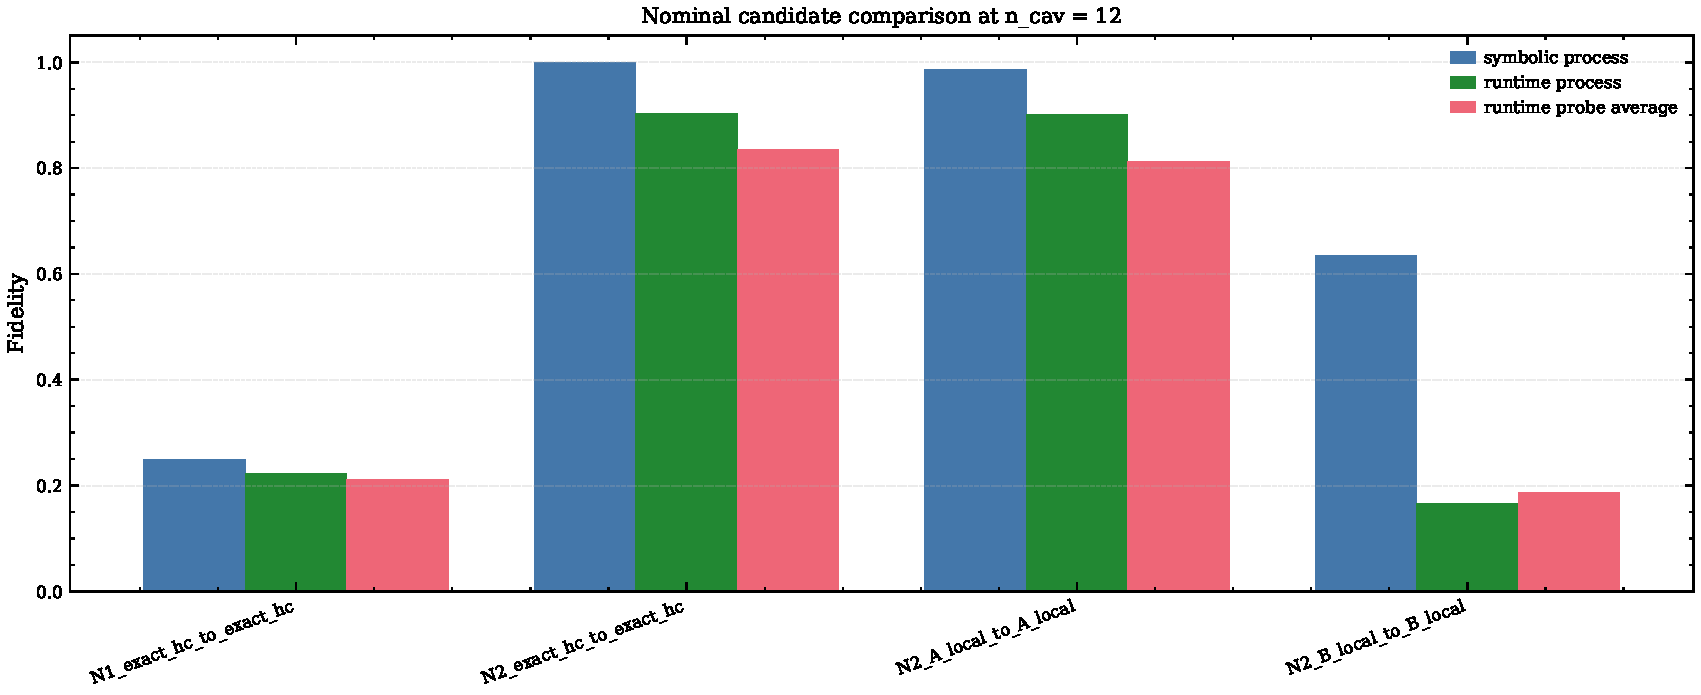
\includegraphics[width=\columnwidth]{../figures/phase5_candidate_comparison.pdf}
  \caption{Phase 5 runtime comparison. The symbolic archive-local focal candidate does not remain the runtime leader once all shortlisted candidates are forced onto replayable implementations. The exact two-wait surrogate family is the best closed-system runtime candidate, while the archive-local surrogate remains competitive and has the strongest final Wigner overlap.}
  \label{fig:comparison}
\end{figure}

\subsection{One-Wait and Direct-Replay Archive References Remain Poor}

The one-wait replay baseline confirms the architectural lower bound. Even after
all local pieces are replaced by replayable implementations,
\texttt{R1\_exact\_runtime\_to\_exact\_runtime} only reaches process fidelity
$0.2234$ and average probe fidelity $0.2120$. It is shorter than the two-wait
families, but it still fails the target badly.

The direct replayable archive reference is more revealing. The
\texttt{B\_local}-based family requires no surrogate for its local block, yet it
performs substantially worse: process fidelity $0.16665$, average probe fidelity
$0.18729$, leakage $0.14324$, and runtime duration \SI{7.912}{\micro\second}.
This confirms that bridge compatibility alone is not enough to justify a
candidate. The replayable archive path remains a useful reference, but not a
competitive synthesis route.

\subsection{Noise Exposure Now Dominates the Practical Interpretation}

The strongest replay-backed candidates are not limited by native entangling time;
they are limited by local-surrogate duration. Each sequence contains three
\SI{1.28}{\micro\second} surrogate blocks plus two native waits and two short
qubit-H replacements, for a total runtime of \SI{4.432}{\micro\second}. Under
the nominal noise model inherited from the earlier hybrid study, the exact
surrogate falls from average probe fidelity $0.83495$ in the closed system to
$0.61448$, while the archive-local surrogate falls to $0.58042$. The runtime
study therefore validates the architecture and the ranking, but it does not yet
validate an experimentally ready pulse schedule.

\section{Validation}

\subsection{Sanity Checks}

Three sanity checks pass. First, the symbolic one-wait family remains pinned near
$0.25$, confirming that one native wait is structurally insufficient. Second,
the symbolic exact two-wait family still reaches unit fidelity to numerical
precision, confirming the architecture-level identity on the logical subspace.
Third, the replay-backed one-wait baseline also remains poor, so the runtime
follow-up does not reopen the one-wait question.

\subsection{Convergence Analysis}

The user explicitly requested stronger truncation checks, so the runtime
shortlist was replayed at $n_{\mathrm{cav}} = 10$, 12, and 14 with
$n_{\mathrm{tr}} = 3$. Table~\ref{tab:convergence} reports the spans of the main
runtime metrics over that sweep. All spans are small enough that the ranking
shift from the symbolic archive-local candidate to the replay-backed exact
surrogate cannot be attributed to truncation error.

\begin{table}[t]
  \centering
  \caption{Metric spans over the runtime truncation sweep $n_{\mathrm{cav}} = 10, 12, 14$.}
  \begin{tabular}{@{} l S[table-format=1.2e-1] S[table-format=1.2e-1] S[table-format=1.2e-1] S[table-format=1.2e-1] @{} }
    \toprule
    Candidate & {$\Delta F_{\mathrm{proc}}$} & {$\Delta \overline{F}_{\mathrm{probe}}$} & {$\Delta L$} & {$\Delta O_{W}$} \\
    \midrule
    R1 exact-runtime & 2.53e-06 & 1.30e-06 & 6.80e-06 & 3.44e-06 \\
    R2 exact-runtime & 7.67e-06 & 9.80e-06 & 1.20e-05 & 7.87e-06 \\
    R2 A-runtime & 2.79e-05 & 6.84e-05 & 6.89e-05 & 1.69e-04 \\
    R2 B-replay & 1.30e-06 & 2.25e-06 & 6.46e-06 & 3.30e-06 \\
    \bottomrule
  \end{tabular}
  \label{tab:convergence}
\end{table}

The convergence figure in Fig.~\ref{fig:convergence} shows the same result
graphically: the runtime metrics are effectively flat across the requested
truncation sweep.

\begin{figure}[t]
  \centering
  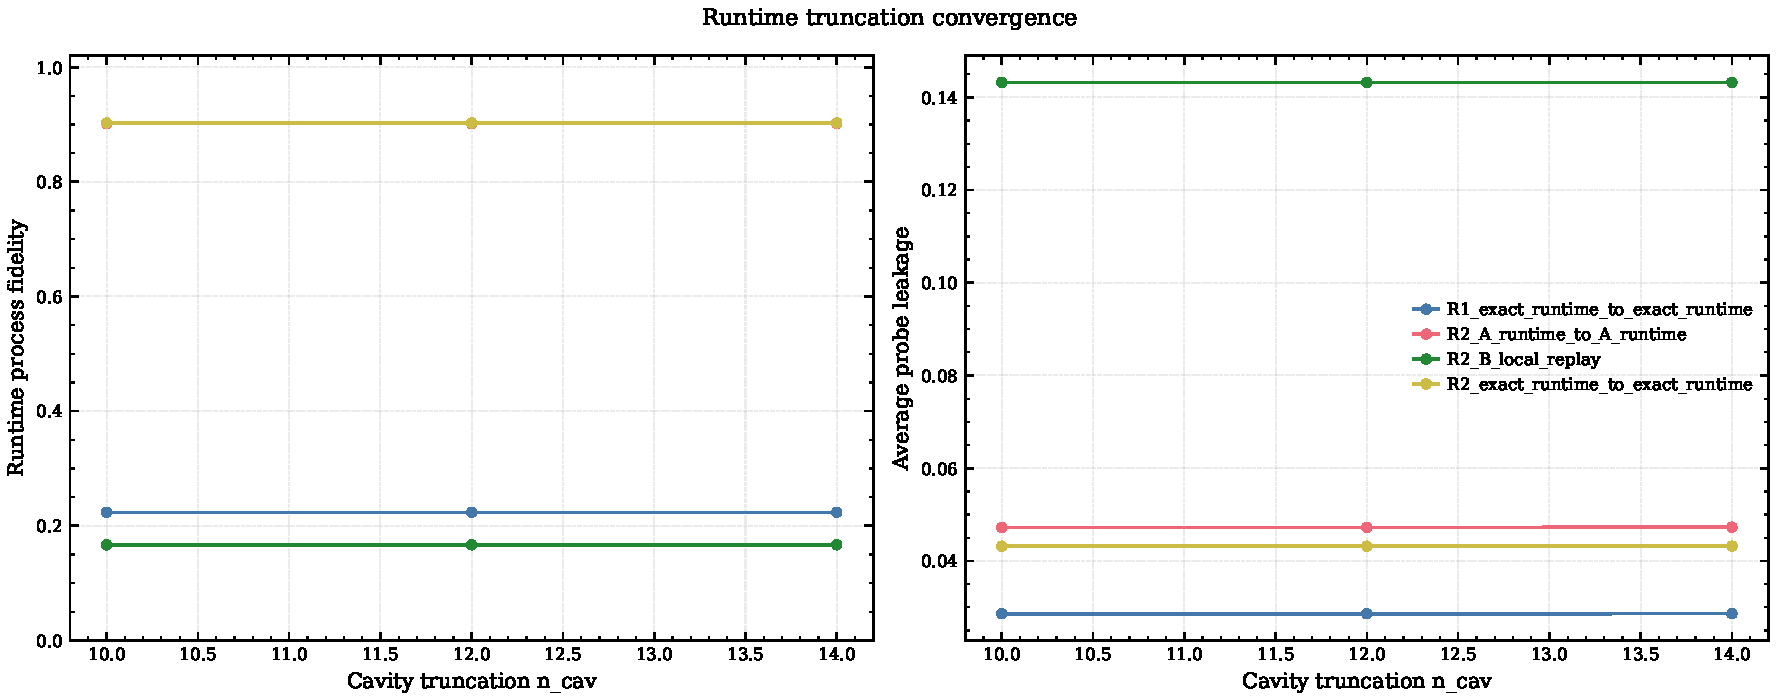
\includegraphics[width=\columnwidth]{../figures/phase5_convergence.pdf}
  \caption{Runtime convergence across $n_{\mathrm{cav}} = 10, 12, 14$. Metric spans are small for every replay-backed candidate, so the ranking shift is not a truncation artifact.}
  \label{fig:convergence}
\end{figure}

\subsection{Literature Comparison}

There is no external published benchmark for this internal target unitary, so
the relevant comparison is internal rather than literature-facing: symbolic
upper bound versus replay-backed realizations under a common device point and
common bookkeeping layer.

\section{Discussion}

The main scientific outcome is not that symbolic analysis was wrong; it is that
symbolic and runtime notions of ``best candidate'' are meaningfully different.
Symbolically, the fully archive-driven two-wait family was the most compelling
experimentally grounded candidate because it preserved the correct architecture
without relying on ideal cavity-H references. Once every candidate is forced
onto a replayable implementation, that ordering changes. The best replay-backed
closed-system candidate is the exact two-wait family with replayable surrogates
for the non-replayable local blocks.

At the same time, the replay-backed archive-local surrogate is not simply worse.
It retains the strongest final Wigner overlap on the probe that is most sensitive
to cavity-structure preservation. This suggests that the two leading runtime
families are emphasizing different physical virtues: the exact surrogate wins on
logical action, while the archive-local surrogate preserves one slice of bosonic
structure slightly better. That difference is small enough to justify keeping
both candidates alive for future optimization, but the present recommendation
still goes to the exact-surrogate family because it wins on the primary logical
metrics and on nominal-noise average probe fidelity.

The more serious practical issue is duration. The native entangling resource is
cheap compared with the replayable local surrogates, so the present runtime
winner is not limited by entangling exposure. It is limited by local-control
overhead. This is why the nominal-noise numbers are mediocre despite reasonably
strong closed-system fidelities. The correct conclusion is therefore skeptical
but useful: the two-wait native architecture is validated, the runtime ranking is
resolved, and the bottleneck has shifted to local replayable control quality and
duration.

The weighted scalar cost deserves one final caution. In the sensitivity sweep,
reducing the infidelity weight by 25 percent makes the one-wait replay baseline
look cheapest even though it plainly fails the target. That is not a scientific
surprise; it is a bookkeeping warning. Any future decision rule should report a
Pareto frontier or enforce a minimum acceptable fidelity before cost is used to
break ties.

\section{Conclusion}

This follow-up converts the earlier symbolic conclusion into a runtime-backed one
and yields four concrete conclusions.

First, one native free-evolution wait remains an architectural lower bound both
symbolically and under replay. Second, the exact two-wait architecture remains
the symbolic upper bound. Third, the best experimentally grounded symbolic
candidate does not remain the runtime leader once replay is enforced: the best
replay-backed closed-system candidate is the surrogate-backed exact two-wait
family, not the surrogate-backed archive-local family. Fourth, the present
runtime winner is not hardware-ready because its \SI{4.432}{\micro\second}
duration drives nominal-noise average probe fidelity down to $0.61448$.

The final recommendation is therefore precise. The correct architecture for this
target is the two-native-wait family, and the current replay-backed focal
candidate is \texttt{R2\_exact\_runtime\_to\_exact\_runtime}. The next study
should optimize local replayable controls, not reopen the symbolic architecture
search.

\section{Limitations and Future Work}

\subsection{Known Limitations}

The runtime-validation gap is closed, but the local replayable surrogates are not
converged. All GRAPE restarts stopped at the iteration limit, and the best local
surrogate fidelities are only $0.94288$ and $0.94762$. This means the present
runtime winner is best within the current surrogate family, not necessarily best
within all replayable local-control strategies.

A second limitation is that noise was only evaluated at one nominal operating
point and one truncation. The nominal-noise calculation is enough to show that
duration is now the dominant practical problem, but it is not enough to claim
robustness under parameter drifts, thermal population, or stronger open-system
effects.

A third limitation is methodological. The scalar weighted cost is convenient for
bookkeeping, but it can mis-rank bad candidates unless a fidelity floor is
imposed. The raw process, probe, leakage, and Wigner metrics should therefore
remain the decision metrics in any future extension.

\subsection{Suggested Improvements}

\begin{itemize}
  \item \textbf{[P1 | HIGH]} Re-optimize the replayable local surrogates with longer optimizer budgets, shorter-duration ansatzes, or smoother parameterizations. The present runtime winner is limited by three \SI{1.28}{\micro\second} surrogate blocks per sequence.
  \item \textbf{[P1 | MEDIUM]} Add a fidelity floor or Pareto filter before scalar cost ranking. The current sensitivity sweep shows that cost alone can prefer the one-wait baseline under weak fidelity weighting.
  \item \textbf{[P2 | MEDIUM]} Expand the noise and robustness study to include amplitude, duration, and dispersive-parameter perturbations in addition to the nominal $T_1/T_2$ point used here.
  \item \textbf{[P2 | MEDIUM]} Compare the current GRAPE surrogates against a direct model-backed \texttt{SNAP} runtime path if one can be added inside \texttt{cqed\_sim} without violating the framework-first rule.
\end{itemize}

\subsection{Open Questions}

Two open questions stand out. Why does the archive-local runtime surrogate retain
the higher final Wigner overlap while losing on process and average probe
fidelity? And can either of the two leading runtime families be compressed below
the current multi-microsecond duration without sacrificing the $\sim 0.90$
closed-system process-fidelity level?

\bibliographystyle{apsrev4-2}
\bibliography{references}

\appendix

\section{Detailed Results and Data}

Table~\ref{tab:appendix_metrics} collects the raw symbolic and runtime metrics at
the reference truncation. These are the values that should be compared directly;
the scalar weighted cost is only a secondary summary.

\begin{table*}[t]
  \centering
  \caption{Raw candidate metrics at $n_{\mathrm{cav}} = 12$, $n_{\mathrm{tr}} = 3$.}
  \begin{tabular}{@{} l S[table-format=1.6] S[table-format=1.6] S[table-format=1.6] S[table-format=1.6] S[table-format=1.6] S[table-format=1.6] S[table-format=1.3] @{} }
    \toprule
    Candidate & {$F_{\mathrm{sym}}$} & {$F_{\mathrm{run}}$} & {$\overline{F}_{\mathrm{probe,run}}$} & {$L_{\mathrm{run}}$} & {$\overline{F}_{\mathrm{probe,noise}}$} & {$O_{W}$} & {$t_{\mathrm{run}}$ (\si{\micro\second})} \\
    \midrule
    R1 exact-runtime & 0.250000 & 0.223401 & 0.211970 & 0.028603 & 0.048006 & 0.512031 & 2.856 \\
    R2 exact-runtime & 1.000000 & 0.902693 & 0.834953 & 0.043177 & 0.614483 & 0.963835 & 4.432 \\
    R2 A-runtime & 0.985681 & 0.901541 & 0.812195 & 0.047255 & 0.580417 & 0.981417 & 4.432 \\
    R2 B-replay & 0.634498 & 0.166650 & 0.187290 & 0.143236 & 0.048845 & 0.259742 & 7.912 \\
    \bottomrule
  \end{tabular}
  \label{tab:appendix_metrics}
\end{table*}

Figure~\ref{fig:bloch_exact_appendix} shows the checkpointed Bloch trajectory for
the runtime winner, and Fig.~\ref{fig:wigner_appendix} compares the final target
and achieved Wigner functions for both leading runtime candidates.

\begin{figure}[t]
  \centering
  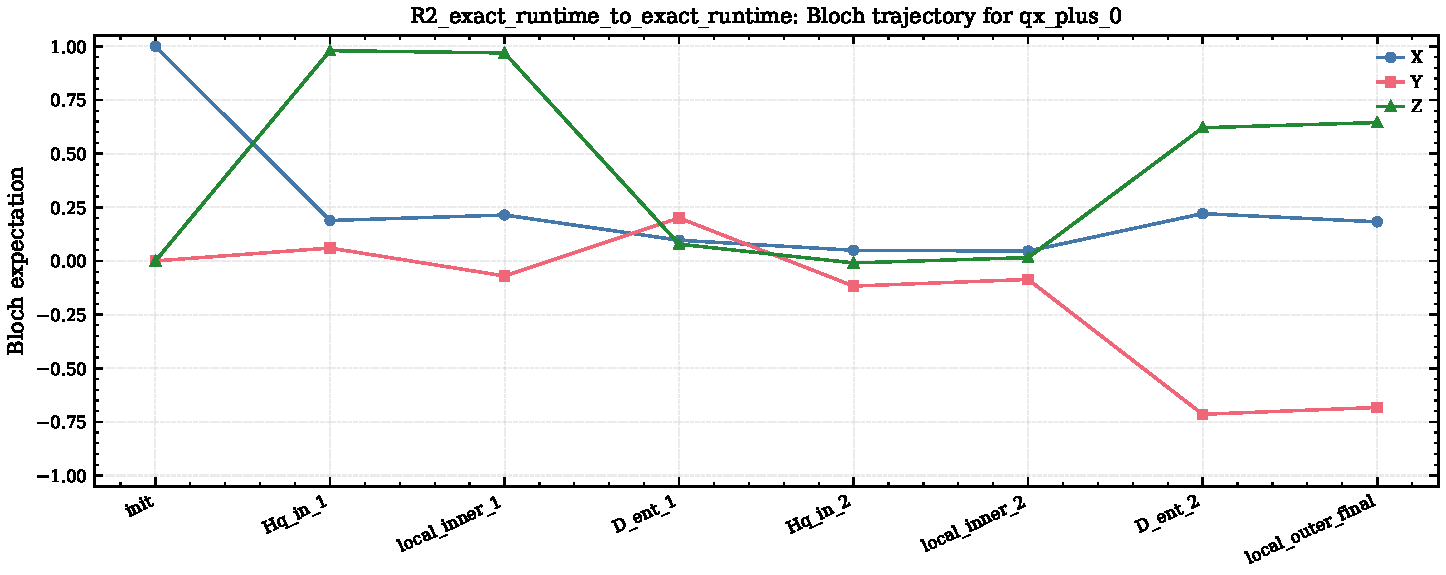
\includegraphics[width=\columnwidth]{../figures/phase5_bloch_R2_exact_runtime_to_exact_runtime_qx_plus_0.pdf}
  \caption{Checkpointed Bloch trajectory for the replay-backed exact two-wait winner on the $\lvert +_x,0 \rangle$ probe.}
  \label{fig:bloch_exact_appendix}
\end{figure}

\begin{figure*}[t]
  \centering
  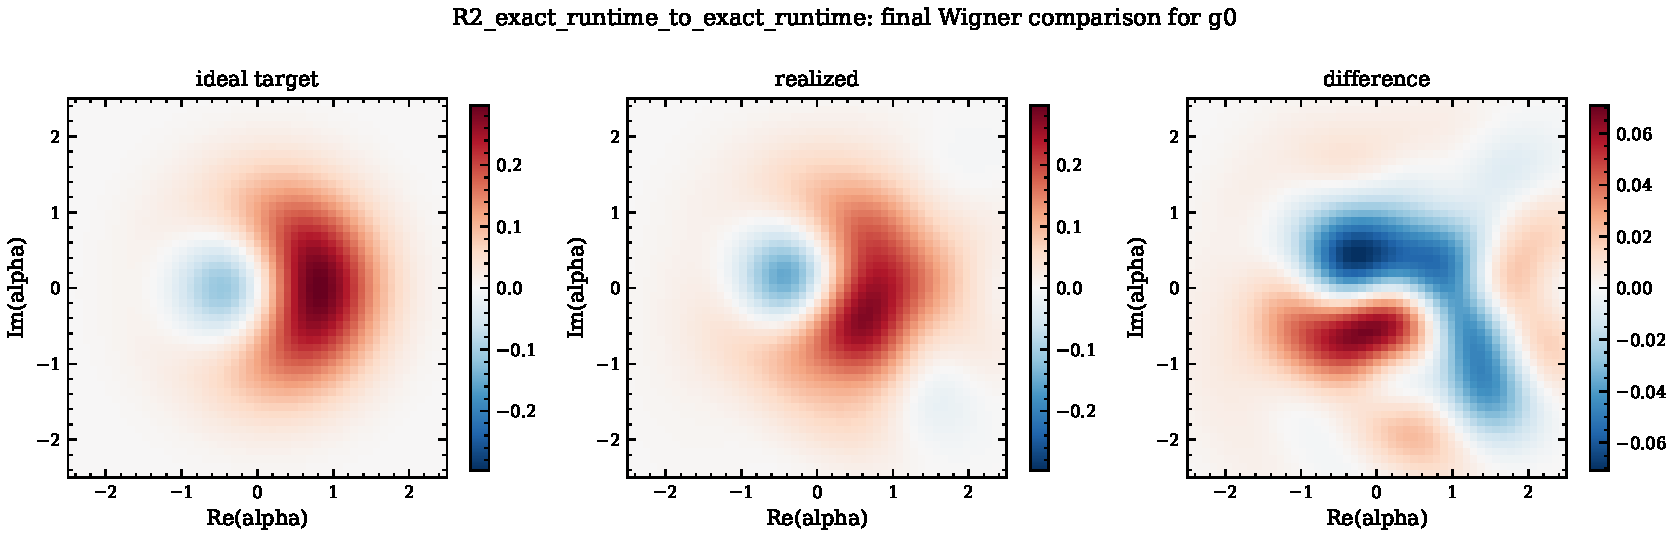
\includegraphics[width=0.48\textwidth]{../figures/phase5_wigner_compare_R2_exact_runtime_to_exact_runtime_g0.pdf}
  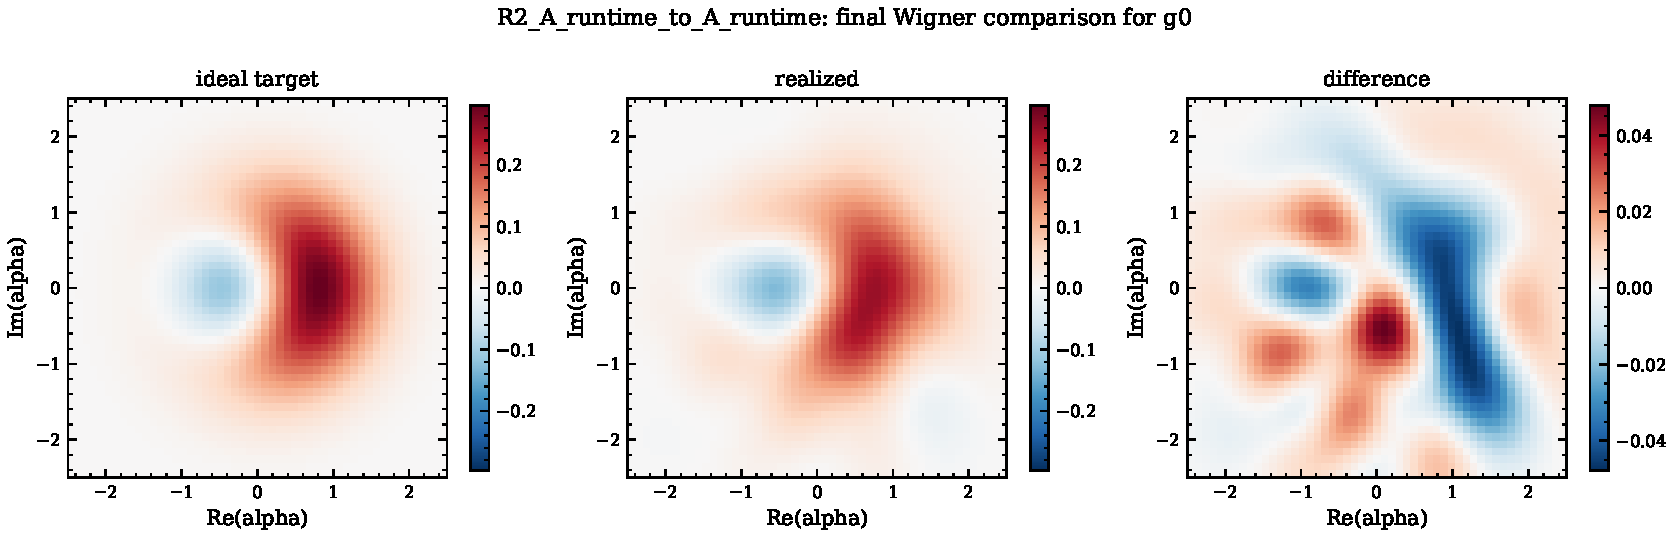
\includegraphics[width=0.48\textwidth]{../figures/phase5_wigner_compare_R2_A_runtime_to_A_runtime_g0.pdf}
  \caption{Final Wigner comparison on the $\lvert g,0 \rangle$ probe for the two leading replay-backed candidates. The archive-local surrogate retains slightly better final Wigner overlap, even though the exact-surrogate family wins on the main logical fidelities.}
  \label{fig:wigner_appendix}
\end{figure*}

Figure~\ref{fig:sensitivity_appendix} records the weight-sensitivity warning. The
one-wait replay baseline can become the scalar-cost winner if the infidelity
term is weakened, so raw metrics must remain primary.

\begin{figure}[t]
  \centering
  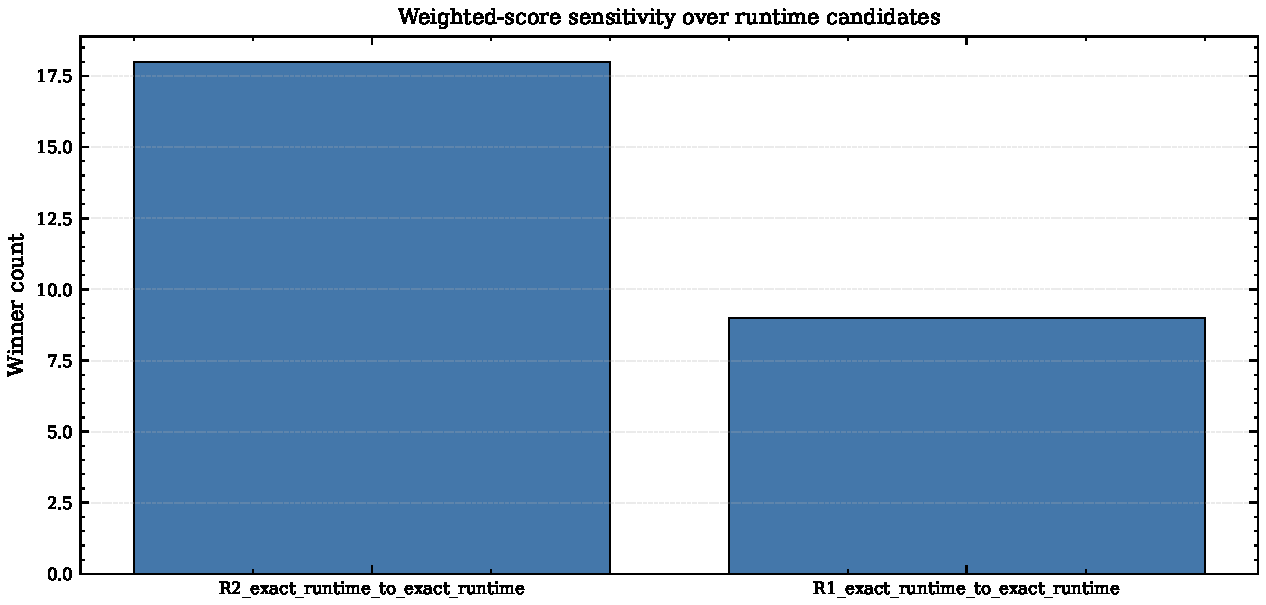
\includegraphics[width=\columnwidth]{../figures/phase5_weight_sensitivity.pdf}
  \caption{Weight-sensitivity sweep for the scalar cost. The one-wait baseline can become the scalar-cost winner if the fidelity term is weakened, which is why the study reports raw metrics rather than relying on a single weighted score.}
  \label{fig:sensitivity_appendix}
\end{figure}

The machine-readable payloads are stored in
\texttt{../data/phase5\_runtime\_validation.json},
\texttt{../data/phase5\_candidate\_comparison.csv},
\texttt{../data/phase5\_runtime\_metrics.csv}, and
\texttt{../data/phase5\_convergence\_table.csv}.

\section{Reproducibility}

\subsection{Optimized Parameters}

\begin{table}[H]
  \centering
  \caption{Replayable local-surrogate parameters at the reference truncation.}
  \begin{tabular}{@{} l S[table-format=1.5] S[table-format=1.2] S[table-format=2.0] S[table-format=1.3] @{} }
    \toprule
    Surrogate & {$F_{\mathrm{nom}}$} & {$t$ (\si{\micro\second})} & {Pulses} & {Restarts} \\
    \midrule
    exact\_hc runtime & 0.94288 & 1.28 & 160 & 3 \\
    A\_local runtime & 0.94762 & 1.28 & 160 & 3 \\
    \bottomrule
  \end{tabular}
  \label{tab:surrogate_params}
\end{table}

The replayable qubit-H replacement is fixed as
$R_{\hat y}(\pi/2)$ followed by $R_{\hat x}(\pi)$, with each pulse lasting
\SI{20}{ns}. Each native entangler is the sequence
qubit rotation -- free evolution -- qubit rotation with total duration
\SI{176}{ns} of free evolution plus two \SI{40}{ns} qubit rotations.

\subsection{Waveform and Pulse Information}

The local-surrogate waveforms are stored in the machine-readable artifacts
\texttt{phase5\_local\_surrogate\_exact\_hc.json},
\texttt{phase5\_local\_surrogate\_exact\_hc\_grape.json},
\texttt{phase5\_local\_surrogate\_A\_local.json}, and
\texttt{phase5\_local\_surrogate\_A\_local\_grape.json} in the
\texttt{../artifacts/} directory. Each surrogate uses four exported control
channels, 40 time slices, and square-envelope pulses on the replay grid.

\subsection{Gate Sequence and Decomposition}

The runtime winner \texttt{R2\_exact\_runtime\_to\_exact\_runtime} uses the
ordered segment sequence
\begin{enumerate}
  \item replayable qubit-H,
  \item exact-H local surrogate,
  \item native entangler,
  \item replayable qubit-H,
  \item exact-H local surrogate,
  \item native entangler,
  \item exact-H local surrogate.
\end{enumerate}
The archive-local runtime candidate uses the same layout but substitutes the
archive-local surrogate for the three local segments. Exact serialized segment
metadata are stored in
\texttt{phase5\_runtime\_candidate\_R2\_exact\_runtime\_to\_exact\_runtime.json}
and
\texttt{phase5\_runtime\_candidate\_R2\_A\_runtime\_to\_A\_runtime.json}.

\subsection{Modeling and Simulation Assumptions}

Symbolic candidates were evaluated on the logical subspace of the dispersive
model using the same device point as the earlier hybrid study. Runtime replay
used $n_{\mathrm{tr}} = 3$ and $n_{\mathrm{cav}} = 10$, 12, and 14, a replay time
step of \SI{2}{ns}, and nominal noise only at the reference truncation. The
noise model uses qubit $T_1 = \SI{30}{\micro\second}$, qubit
$T_2 = \SI{20}{\micro\second}$, pure dephasing inferred from those values, and
cavity decay $\kappa = 1/T_{1,c}$ with $T_{1,c} = \SI{250}{\micro\second}$.

\subsection{Reproduction Procedure}

To reproduce the Phase 5 results from the study folder:
\begin{enumerate}
  \item run \texttt{python scripts/phase5\_runtime\_validation.py} from
  \texttt{studies/hybrid\_unitary\_native\_entangling\_evolution/};
  \item confirm that the script writes the Phase 5 CSV tables into
  \texttt{data/}, the surrogate and runtime-decomposition artifacts into
  \texttt{artifacts/}, and the runtime comparison, convergence, Bloch, and
  Wigner figures into \texttt{figures/};
  \item verify agreement by checking that the leading runtime candidate is
  \texttt{R2\_exact\_runtime\_to\_exact\_runtime} with process fidelity near
  $0.90269$ and that the convergence spans in
  \texttt{phase5\_convergence\_table.csv} remain at or below the values reported
  in Table~\ref{tab:convergence}.
\end{enumerate}

\subsection{Saved Artifacts}

The key machine-readable artifacts are:
\begin{itemize}
  \item \texttt{phase5\_local\_surrogate\_exact\_hc.json}: exported replayable pulses and metadata for the exact-H local surrogate,
  \item \texttt{phase5\_local\_surrogate\_exact\_hc\_grape.json}: full GRAPE payload for that surrogate,
  \item \texttt{phase5\_local\_surrogate\_A\_local.json}: exported replayable pulses and metadata for the archive-local surrogate,
  \item \texttt{phase5\_local\_surrogate\_A\_local\_grape.json}: full GRAPE payload for that surrogate,
  \item \texttt{phase5\_runtime\_candidate\_R2\_exact\_runtime\_to\_exact\_runtime.json}: serialized replay decomposition for the runtime winner,
  \item \texttt{phase5\_runtime\_candidate\_R2\_A\_runtime\_to\_A\_runtime.json}: serialized replay decomposition for the archive-local runtime finalist,
  \item \texttt{phase5\_runtime\_candidate\_R2\_B\_local\_replay.json}: serialized direct replay decomposition for the archive reference.
\end{itemize}

These files are sufficient for a future agent to inspect the runtime candidate
structure, reload pulse metadata, and reproduce the ranking without reverse
engineering the report text.

\end{document}